\documentclass[UTF8,10pt,a4paper,fontset=fandol]{ctexart}
\usepackage[margin=19mm]{geometry}
\usepackage{graphicx,booktabs,tabularx,hyperref,float}
\hypersetup{hidelinks}
\setlength{\parindent}{2em}
\setlength{\parskip}{3pt}
\setlength{\textfloatsep}{10pt}
\setlength{\intextsep}{8pt}
\widowpenalty=10000
\title{因子流动性测试报告}\date{}\author{}
\begin{document}
{\Large\bfseries 因子流动性测试报告}\par
本次输入因子：F000001收益率因子（N20合法订单代表账户），测试期为2024-01-02至2024-08-30。目前已完成4个资金账户的全期回放，并核对了现金、持仓和净值。其中，0个资金档完成了全部当日事前合法订单，4个未达到这一要求，0个仍待核实。目前还没有找到满足这一标准的资金档，下面结合未完成计划说明原因。新增冲击按参数情景在成交前联动现金与数量；模型尚未经公司真实执行记录校准，收益和完成表现均取连续账户重跑。\section*{合法订单与权重目标偏差}本报告的100\%只指事前合法订单完成，不表示G1等权目标被100\%实现。G1成员、权重和H20日程保留，理论净需求向下投影为合法数量，不重新分配被舍去的权重。零合法计划仍保留为目标覆盖记录；未知资料继续待核。\begin{table}[H]\centering\scriptsize\begin{tabular}{lllrrrr}\toprule N & 情景 & 资金 & 舍入差额(万) & 零计划数 & 零计划差额(万) & 未建仓目标数\\\midrule N20 & 常规 & 1000万元 & 639.76 & 569 & 241.95 & 191 \\
N20 & 常规＋冲击成本 & 1000万元 & 640.89 & 570 & 241.81 & 191 \\
N20 & 扫板 & 1000万元 & 640.32 & 568 & 242.02 & 191 \\
N20 & 扫板＋冲击成本 & 1000万元 & 639.57 & 570 & 241.96 & 191 \\\bottomrule\end{tabular}\end{table}舍入差额按每个目标批次中首次计划或零计划的参考价累计，不累加次日重试和已完成后的日记录，也不是收益损失。未建仓目标数指正权重、无持仓权益且合法计划为零的首次目标。表列各组最低已测资金；全部资金及未建仓目标金额见plan\_rounding\_summary.csv。

\begin{table}[H]\centering\small
\begin{tabular}{llllr}\toprule
回看期 & 情景 & 最大已测通过 & 更高未通过档 & 已测档数\\\midrule
N20 & 常规 & 尚无 & 尚无 & 1 \\
N20 & 扫板 & 尚无 & 尚无 & 1 \\
N20 & 常规＋冲击成本 & 尚无 & 尚无 & 1 \\
N20 & 扫板＋冲击成本 & 尚无 & 尚无 & 1 \\
\bottomrule\end{tabular}
\end{table}
表中的“最大已测通过”是本次窗口和执行条件下，已经逐档验证通过的最大资金。未测区间和待核实账户仍需继续检查；“尚无”表示还没有找到通过档，而不是把容量记为零。



\section*{因子和实验设置}
使用过去N个交易日复权价格变化的原始信号，经原批次预处理后取G1并等权配置。不同N只改变原回看期版本，不重选参数。

N表示因子的回看期，H表示调仓间隔，两者都按交易日计算。

N20：H=20，每20个交易日调仓；输入为已生成的目标持仓；沿用输入分组，取G1。

各资金档沿用同一套G1等权和H20规则。09:35先以账户净值乘目标权重、除参考价，减去实际持仓和应收权益，得到理论净需求，再按申报下限、增量和卖方整仓零股规则向下确定合法订单。舍入差额保留，不把资金或成交条件不足转成零目标。账户现金、持仓和权益连续保留到下一交易日。

本报告账户的金融规则版本为g1-0935-legal-plan-impact-20261116-v5。09:35目标定量采用事件状态参考价：仅使用决策前已读取的[09:34,09:35)窗口中的当日早盘观测，正常静默超过30秒本身不使参考价失效。最新观测无效时不退回更早有效报价，已知复牌后仍需新的合格观测。窗口内没有参考观测不等于当日没有行情。

订单发出后，经过设定的报单延迟，才在后续合格快照上模拟成交。当时只能成交一部分，就先记下这部分成交并保留余单。所有买卖共用同一个现金账户：买单预留的资金不能再分给其他订单，卖单实际成交后才增加可用现金。未完成的目标和后续调仓都从这一实际账户状态继续计算。

本报告只展示初始资金为1000万元的代表账户，各情景分别连续回放；不据此推断其他资金规模的容量。

常规情景的成交量参与率为10\%。指令生效后，程序根据后续合格快照中观察到的新增成交量，逐步释放该股票的成交额度。同一股票的多笔订单共同使用这份额度，盘口中可见的对手方数量也会限制成交。此外，策略在该股的累计成交金额最多占截至当时市场已公布累计成交额的10\%。

扫板是另一种执行情景：距涨跌停幅度差1个百分点时触发，即上涨9\%／19\%时买入，下跌9\%／19\%时卖出，对应10\%／20\%涨跌幅制度。触发后，假设后续观察到的市场新增成交量全部可供本策略使用，买入按官方涨停价、卖出按官方跌停价记账。现金和可卖量仍受账户约束。原扫板基线采用乐观成交假设，没有额外冲击成本；启用冲击的情景另列，均未模拟真实排队竞争。

本情景的通过条件是：测试期内，每笔事前确定的正数量合法订单均在计划当天100\%完成。合法计划量在09:35按理论净需求和申报数量规则确定，不按资金、可卖量、盘口或后来成交量缩小。非零订单未发出或仍有余量都未通过，后日重试不能修复原日失败。零合法计划单列目标偏差，不叫达成目标；全部为零而没有正合法订单的账户不能证明容量通过。资料不足的目标和账户仍待核。

报告同时展示模型收益和按金额衡量的完成情况。模型收益等于期末净值除以初始资金再减一。基线佣金税费为0；额外模型冲击单独列示，启用时在成交前进入现金和数量计算。盘口价差、跨档及扫板价格成本已包含在成交金额中，不再重复扣除。金额完成率用计划时的参考价把买卖股数换算成金额，买入和卖出都按正数合计；图中展示完成情况最差的一天。容量是否通过仍按逐笔100\%判断。

\section*{资金规模与收益、成交}
\begin{figure}[H]\centering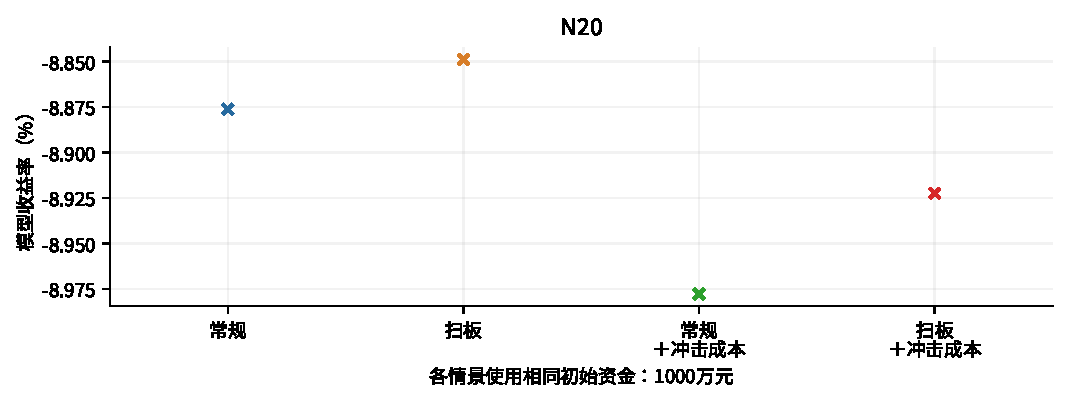
\includegraphics[width=.82\linewidth]{figures/capital_return.pdf}
\caption{已测资金规模下各情景的全期模型收益。点表示已完成回放并核账的资金档，连线不代表未测区间通过；冲击情景使用扣除额外模型成本后的账户净值。}\end{figure}
\begin{figure}[H]\centering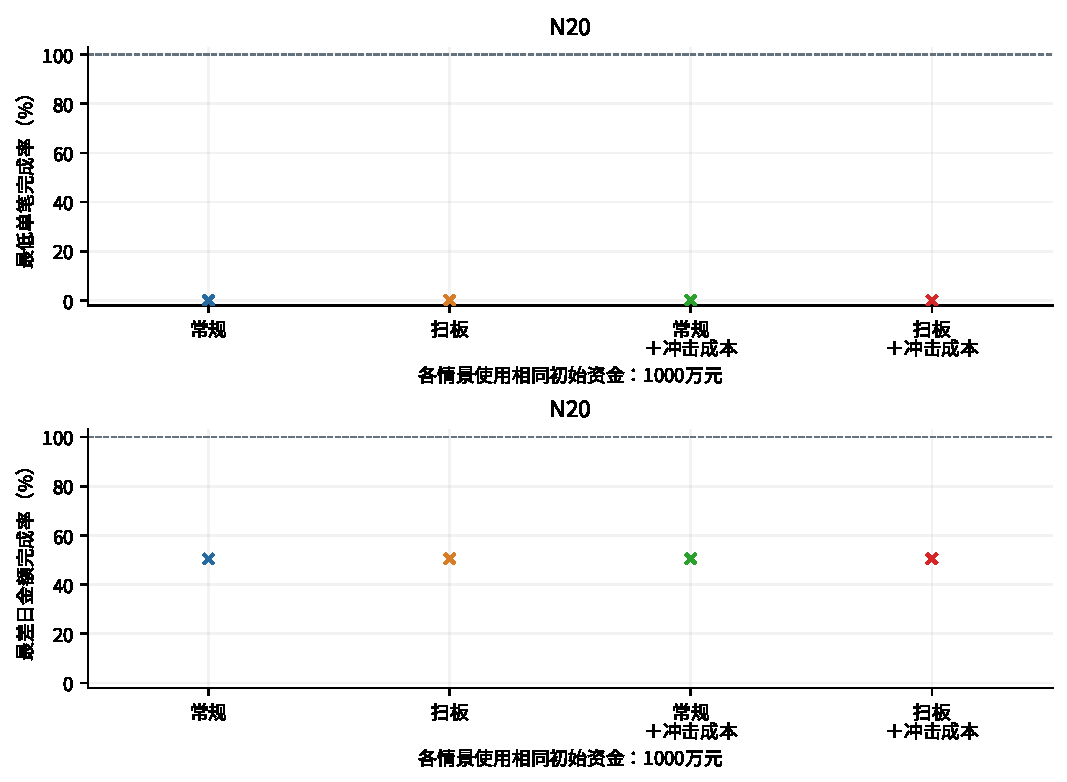
\includegraphics[width=\linewidth]{figures/capital_completion.pdf}
\caption{资金与最低单笔完成率、最差交易日金额完成率。颜色区分执行情景；圆点通过、叉号未通过、三角待核实。}\end{figure}
\section*{额外冲击成本与账户结果}本情景估计的是可见盘口成本之外的额外经济成本。背景成交价仍来自实际档价或原扫板官方限价；不把经济成本折算价称为交易所成交价，不在涨跌停外成交，也不通过截价恢复原成交保证。扫板的100\%后续有效新增量可用仍是原定义的情景假设，新增成本没有复原真实排队或其他交易者反应。设同账户、同证券、方向和交易日的累计执行金额为$X$，本次成交金额为$\Delta X$，当时已知市场累计金额为$M$，额外成本为$k[(X+\Delta X)^{3/2}-X^{3/2}]/\sqrt{M}$。所有金额单位为元，$k=(b/10000)/\sqrt{0.1}$；本报告参数b为5基点，表示在固定M下累计执行额占已知市场额10\%时的累计平均成本量级，属于敏感性假设，未采用库默认系数作为A股实证值。同一母单拆成子单不清空累计金额；实际减慢执行改变所观察的市场量时，成本也可能变化。盘中不使用未来全天成交额。\begin{figure}[H]\centering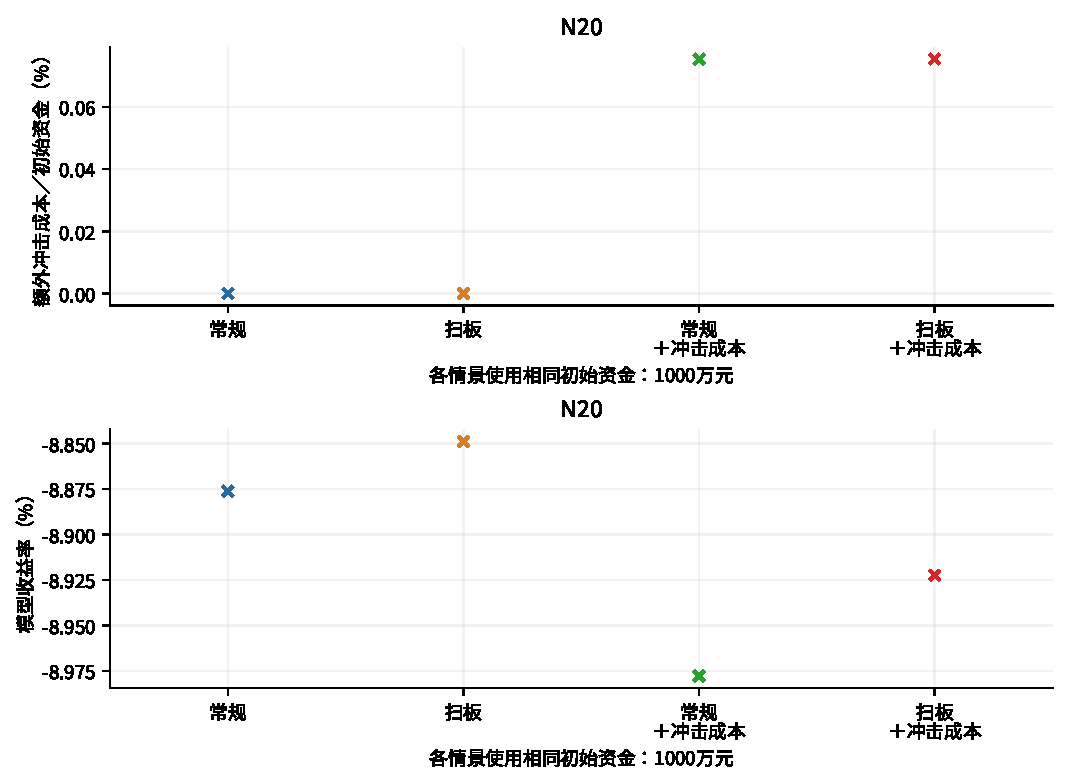
\includegraphics[width=\linewidth]{figures/capital_impact.pdf}\caption{额外冲击成本占初始资金及冲击后的全期模型收益。不同账户路径的收益差不等于直接冲击费用；未设置经济容量阈值。}\end{figure}\begin{table}[H]\centering\scriptsize\begin{tabular}{lllrrrr}\toprule N & 情景 & 资金 & 盘口成本(万) & 扫板价差(万) & 额外冲击(万) & 佣金税费(万)\\\midrule N20 & 常规 & 1000万元 & 待核 & 待核 & 未启用 & 0 \\
N20 & 扫板 & 1000万元 & 待核 & 待核 & 未启用 & 0 \\
N20 & 常规＋冲击成本 & 1000万元 & 11.26 & 0 & 0.75 & 0 \\
N20 & 扫板＋冲击成本 & 1000万元 & 11.23 & 0.06 & 0.75 & 0 \\\bottomrule\end{tabular}\end{table}盘口成本和扫板价差相对当时背景中价计量，已包含于成交金额；额外冲击与佣金税费独立计入现金。表列各组最低已测资金，全部资金见图源表。\section*{原计划完成时间}以原计划日的固定正数量需求为分母，30／60分钟均为交易分钟，扣除午休。跨日重试不新增计划，也不改写原日结果。未完成计划和缺时间证据的计划保留在分母；待定量目标另列在随附表。下表列各组最低已测资金，全部资金及已完成计划耗时分位数见图源表。\begin{table}[H]\centering\scriptsize\begin{tabular}{lllrrrrr}\toprule N & 情景 & 资金 & 正计划 & 30分全成 & 60分全成 & 当日未成 & 时间待核\\\midrule N20 & 常规 & 1000万元 & 11508 & 11476 & 11480 & 26 & 0 \\
N20 & 常规＋冲击成本 & 1000万元 & 11507 & 11475 & 11479 & 26 & 0 \\
N20 & 扫板 & 1000万元 & 11509 & 11491 & 11493 & 15 & 0 \\
N20 & 扫板＋冲击成本 & 1000万元 & 11507 & 11489 & 11491 & 15 & 0 \\\bottomrule\end{tabular}\end{table}
\section*{哪些交易没有完成}
\begin{table}[H]\centering\scriptsize\begin{tabular}{lllllrrr}\toprule 证券 & 日期 & N & 情景 & 资金 & 计划量 & 成交量 & 余量\\\midrule 证券1 & 06-17 & N20 & 常规 & 1000万元 & 2,900 & 0 & 2,900 \\
证券2 & 04-16 & N20 & 常规 & 1000万元 & 1,400 & 0 & 1,400 \\
证券3 & 06-18 & N20 & 扫板 & 1000万元 & 22,300 & 0 & 22,300 \\
证券4 & 06-18 & N20 & 扫板 & 1000万元 & 26,300 & 0 & 26,300 \\
证券1 & 06-17 & N20 & 常规＋冲击成本 & 1000万元 & 2,900 & 0 & 2,900 \\
证券2 & 04-16 & N20 & 常规＋冲击成本 & 1000万元 & 1,400 & 0 & 1,400 \\
证券3 & 06-18 & N20 & 扫板＋冲击成本 & 1000万元 & 22,200 & 0 & 22,200 \\
证券4 & 06-18 & N20 & 扫板＋冲击成本 & 1000万元 & 26,200 & 0 & 26,200 \\\bottomrule\end{tabular}\end{table}\begin{table}[H]\centering\scriptsize\begin{tabular}{llrrrrr}\toprule 证券 & 日期 & 前20日均额(万) & 当日额(万) & 当日/均额 & 扫板 & 扫板成交量\\\midrule 证券1 & 06-17 & 6,731.74 & 5,359.61 & 0.8 & 否 & 0 \\
证券2 & 04-16 & 10,916.23 & 3,982.33 & 0.36 & 否 & 0 \\
证券3 & 06-18 & 4,366.27 & 170.7 & 0.04 & 否 & 0 \\
证券4 & 06-18 & 352.46 & 185.77 & 0.53 & 否 & 0 \\
证券1 & 06-17 & 6,731.74 & 5,359.61 & 0.8 & 否 & 0 \\
证券2 & 04-16 & 10,916.23 & 3,982.33 & 0.36 & 否 & 0 \\
证券3 & 06-18 & 4,366.27 & 170.7 & 0.04 & 否 & 0 \\
证券4 & 06-18 & 352.46 & 185.77 & 0.53 & 否 & 0 \\\bottomrule\end{tabular}\end{table}\begin{figure}[H]\centering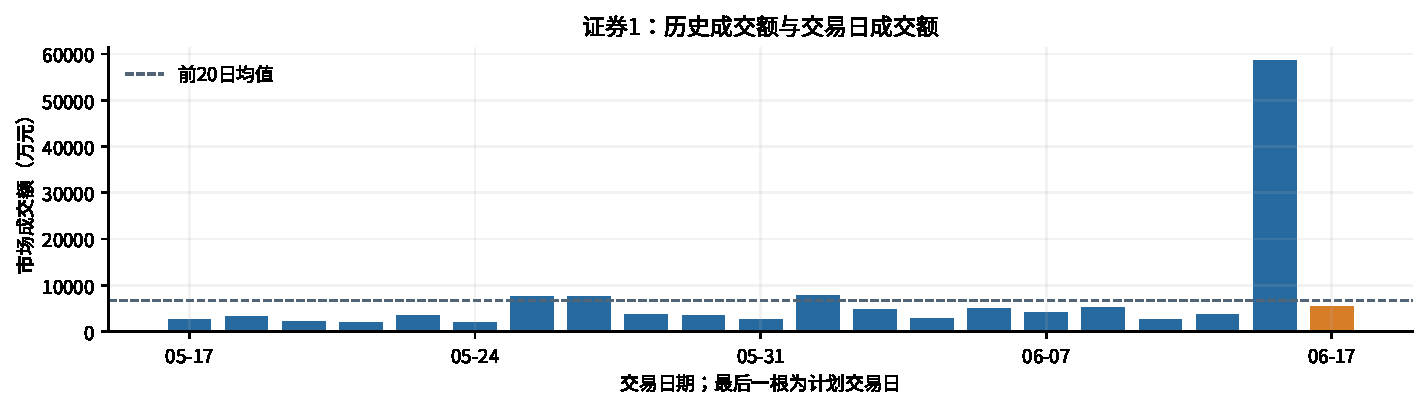
\includegraphics[width=\linewidth]{figures/turnover_case.pdf}\caption{同一证券在此前20个交易日和计划交易日的成交额，虚线为前20日均值。}\end{figure}图表用证券编号展示，实际股票代码和逐笔明细保存在私有结果目录。

前20日均成交额用来观察股票平时的交易活跃度，当日成交额则帮助判断计划交易日是否明显放量或缩量。均值取此前20个官方交易日，已确认零成交的日期也计入；历史资料不足时留空。当日成交额用于事后解释，盘中下单不会提前知道这个数。是否因历史放量而入选，还需要结合原选股规则判断。

案例1为N20的常规＋冲击成本账户，资金1000万元，2024-01-11原计划2800股／份，当日实际成交2800，剩余0。该计划没有已保存的扫板触发证据。额外模型冲击成本0.74元，单独进入现金，不改变官方成交价格。\begin{figure}[H]\centering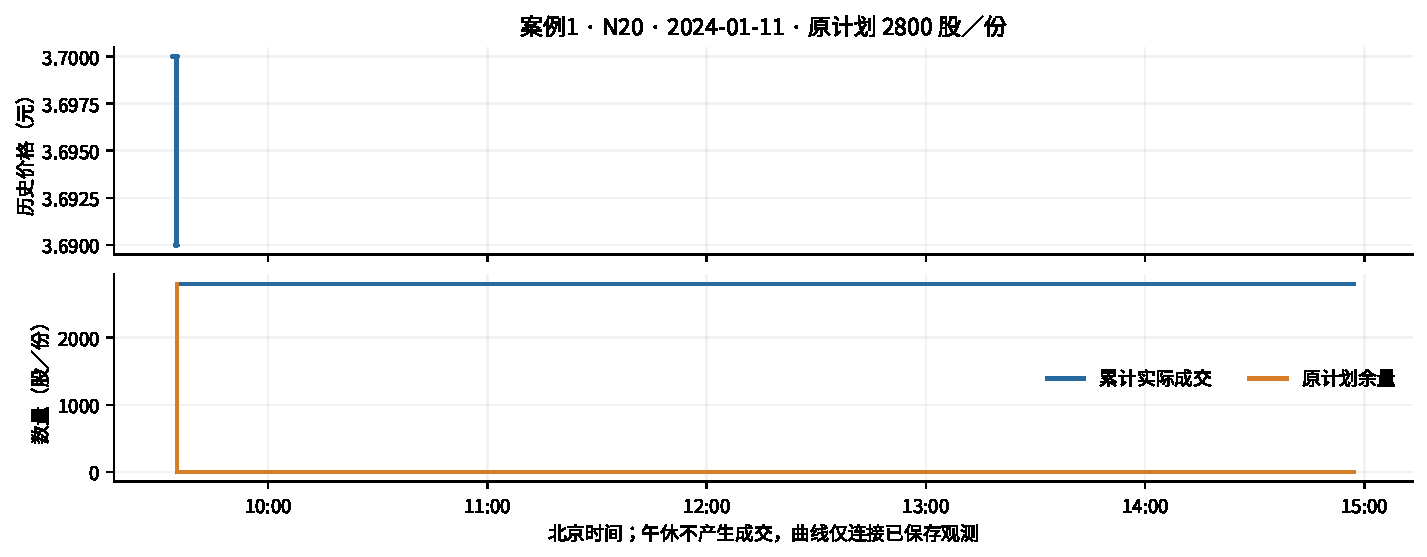
\includegraphics[width=.85\linewidth]{figures/intraday_1.pdf}\caption{实际历史观测与该账户的原计划执行。案例说明执行过程，不代表发生频率；不同情景各用自己的计划与账户路径。}\end{figure}案例2为N20的扫板＋冲击成本账户，资金1000万元，2024-01-11原计划500股／份，当日实际成交500，剩余0。扫板首次触发于09:35:00。其中实际扫板成交500股／份。额外模型冲击成本0.08元，单独进入现金，不改变官方成交价格。\begin{figure}[H]\centering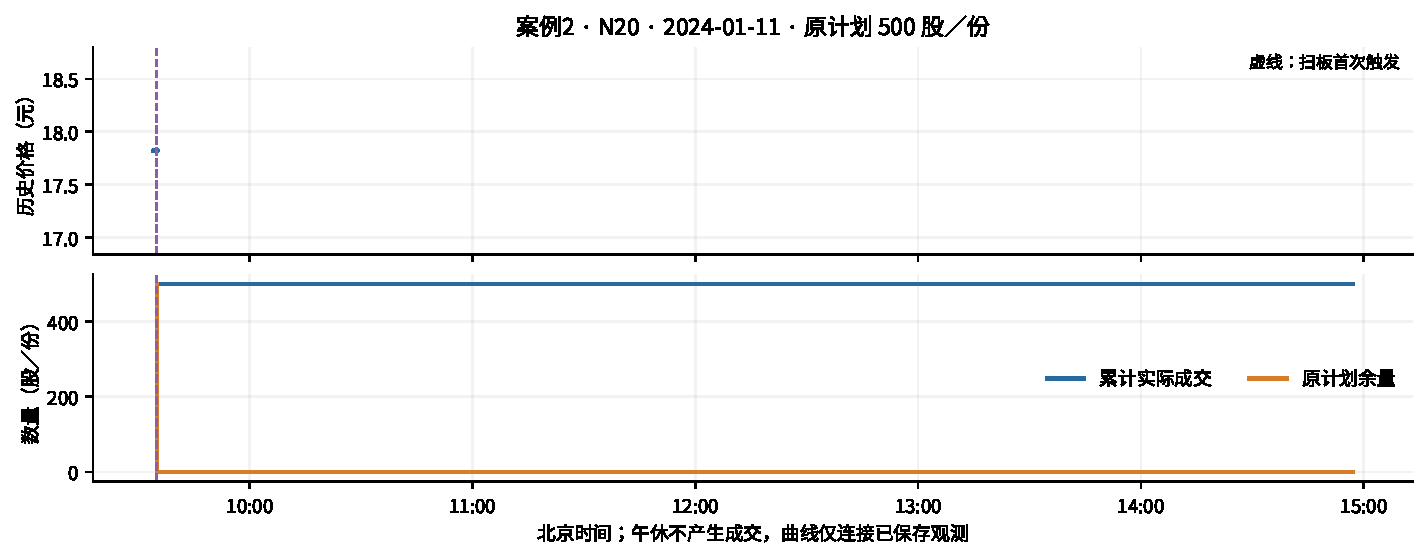
\includegraphics[width=.85\linewidth]{figures/intraday_2.pdf}\caption{实际历史观测与该账户的原计划执行。案例说明执行过程，不代表发生频率；不同情景各用自己的计划与账户路径。}\end{figure}案例3为N20的常规＋冲击成本账户，资金1000万元，2024-06-17原计划2900股／份，当日实际成交0，剩余2900。该计划没有已保存的扫板触发证据。额外模型冲击成本0.00元，单独进入现金，不改变官方成交价格。\begin{figure}[H]\centering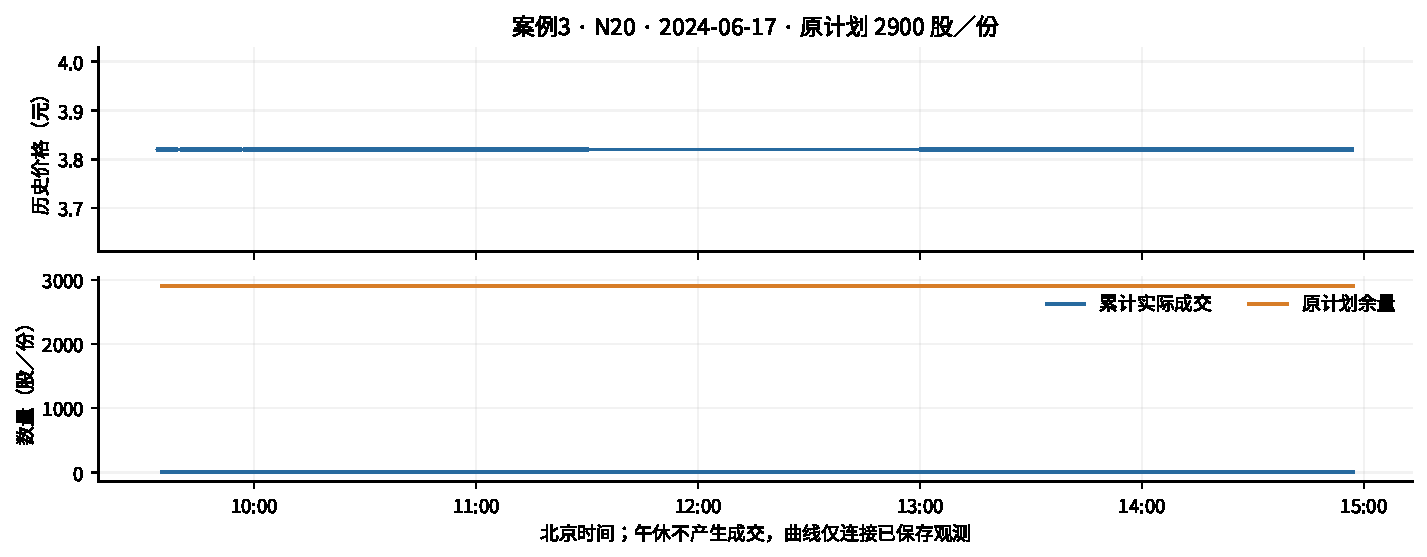
\includegraphics[width=.85\linewidth]{figures/intraday_3.pdf}\caption{实际历史观测与该账户的原计划执行。案例说明执行过程，不代表发生频率；不同情景各用自己的计划与账户路径。}\end{figure}

\section*{停牌、涨跌停和其他限制}
下表把交易中遇到的限制分开列出，帮助解释哪些计划没有完成。每笔原始计划只计一次，次日继续交易不会再算一笔新计划。同一计划可能同时遇到几种限制，因此各行数量不能相加。

每个N和情景选一个代表资金档，优先选择资金最小的未完成档。本表使用：N20/常规 1000万元、N20/扫板 1000万元、N20/常规＋冲击成本 1000万元、N20/扫板＋冲击成本 1000万元。各账户分别计数，同一股票在不同账户中的计划会分别列入。\begin{table}[H]\centering\small\begin{tabular}{lrrr}\toprule 遇到的情况 & 涉及计划 & 仍有未成交量 & 数量待核\\\midrule 有明确停牌记录 & 108 & 0 & 108 \\
停牌记录的日内时段未核实 & 108 & 0 & 108 \\
涨跌停资料或状态待核实 & 60 & 0 & 60 \\
触发扫板假设 & 66 & 0 & 0 \\
记录过现金约束 & 18258 & 0 & 0 \\
公司行动或权益政策约束 & 2088 & 0 & 2088 \\
参考价或行情资料待核实 & 120 & 20 & 24 \\
决策前最新观测不合格 & 24 & 0 & 24 \\
未完成条件未归入上述类别 & 62 & 62 & 0 \\\bottomrule\end{tabular}\end{table}

停牌记录涉及108笔计划。其中108笔还缺少明确的起止时间，需要补齐才能判断哪些时段可以交易；另有0笔计划的停牌状态尚待核实。

现金不足记录的是交易过程中曾遇到的限制；条件恢复后，订单仍可继续执行。

分红送转等权益处理与行情资料问题分别列出。缺少参考价、行情或交易状态时，先保留待核状态，补齐资料后再判断成交条件。参考价采用前文所述的本报告账户规则，正常静默本身不证明数据损坏。

记录为关键事件排除的目标，按整个研究窗口的公司行动资料，在各账户共同现金起点固定排除。排除名单可能使用目标日之后才公告的事件资料，因此结果描述的是这一固定排除范围下的研究情景，不能解释为目标当日已知信息的筛选，也不表示当日缺少L2行情。涉及零碎股分配时，输入准备阶段按每股比例和来源分配要求统一判断，尚未结合各账户登记日的实际持股逐一判断应得新增股份是否恰为整数。原目标权重不重新分配，相关待核目标不计为成交完成。

\end{document}
